% =====================================================================
% Laporan Tugas — Workshop Deep Learning (Teknik Telekomunikasi ITERA)
% Studi Ablasi RNN, LSTM, GRU vs ANN untuk Prediksi Trafik Seluler
%
% Format IEEE conference dua kolom, MAKSIMAL 6 HALAMAN termasuk referensi.
% Compile: pdflatex main && bibtex main && pdflatex main && pdflatex main
%
% TEKS MERAH [ ... ] = BELUM ADA DATA / HARUS KALIAN ISI. Cari "\isi{" untuk
% menemukan semuanya, lalu ganti dengan isi sebenarnya. Hapus makro \isi di akhir.
% =====================================================================
\documentclass[conference,a4paper]{IEEEtran}
\IEEEoverridecommandlockouts

\usepackage[indonesian]{babel}
\usepackage[utf8]{inputenc}
\usepackage[T1]{fontenc}
\usepackage{cite}
\usepackage{amsmath,amssymb}
\usepackage{graphicx}
\usepackage{booktabs}
\usepackage{siunitx}
\usepackage{xcolor}
\usepackage[hidelinks]{hyperref}
\graphicspath{{gambar/}{hasil/}}

% Penanda isian yang belum final (tampil merah)
\newcommand{\isi}[1]{\textcolor{red}{\textbf{[#1]}}}

\begin{document}

\title{Studi Ablasi RNN, LSTM, dan GRU dibandingkan ANN untuk Prediksi Trafik Seluler Kota Milan}

\author{
\IEEEauthorblockN{Zahra Shakilla}
\IEEEauthorblockA{NIM 124400021\\
Teknik Telekomunikasi, ITERA\\
zahra.124400021@student.itera.ac.id}
}

\maketitle

\begin{abstract}
Operator seluler memerlukan prakiraan trafik per sel untuk perencanaan kapasitas. Laporan ini membandingkan ANN, RNN, LSTM, dan GRU untuk memprediksi aktivitas internet per jam pada data Telecom Italia di kotak Duomo, Milan, lalu mengukur seberapa besar hasil bergantung pada \textit{hyperparameter} melalui studi ablasi: lima faktor wajib (panjang jendela, ukuran \textit{hidden}, jumlah lapisan, \textit{learning rate}, kelompok fitur) dan empat faktor pilihan (\textit{batch}, \textit{dropout}, \textit{loss}, \textit{clipping}), masing-masing dilatih dengan tiga seed. Pada konfigurasi acuan, RNN dan GRU (test MAE $229{,}6 \pm 5{,}1$ dan $237{,}2 \pm 9{,}3$) lebih baik daripada ANN ($309{,}9 \pm 5{,}9$) dan jauh di bawah baseline naif terbaik ($467{,}6$). ANN memburuk pada jendela panjang (val MAE $211{,}5$ pada $W=6$ menjadi $298{,}2$ pada $W=168$), sedangkan model rekuren hampir tidak terpengaruh; GRU kecil (3.969 parameter) mengalahkan ANN besar (38.273 parameter). Konfigurasi terbaik yang dipilih dengan val MAE adalah GRU dengan \textit{hidden} 128 (val MAE $188{,}7 \pm 4{,}2$; test MAE $220{,}3 \pm 10{,}6$, turun $7{,}1$\,\% dari acuan GRU). Menggabungkan semua nilai terbaik per faktor justru lebih buruk daripada satu faktor terbaik pada keempat model, yang menandakan interaksi antar faktor. Pada minggu Natal, galat semua model naik sekitar dua hingga tiga kali lipat karena pola Natal tidak ada di data latih. Di Navigli (Darsena), urutan model berubah (GRU dan RNN terbaik, LSTM di bawah ANN) dan konfigurasi terbaik dari Duomo tidak konsisten lebih baik pada minggu uji.
\end{abstract}

\begin{IEEEkeywords}
prediksi trafik seluler, RNN, LSTM, GRU, studi ablasi
\end{IEEEkeywords}

% ---------------------------------------------------------------------
\section{Pendahuluan}
Prakiraan trafik per sel membantu operator merencanakan kapasitas dan mengatur sumber daya jaringan. Trafik seluler berpola harian dan mingguan, sehingga model sekuensial seperti RNN, LSTM \cite{hochreiter1997lstm}, dan GRU \cite{cho2014gru} wajar dibandingkan dengan ANN yang menerima jendela masukan sebagai satu vektor. Namun, hasil perbandingan satu konfigurasi belum menunjukkan seberapa besar kesimpulan bergantung pada pilihan \textit{hyperparameter}. Studi ablasi mengubah satu faktor sekali waktu dari konfigurasi acuan untuk menjawab hal itu. Kontribusi laporan ini: (i) ablasi lima faktor wajib dan beberapa faktor pilihan pada empat model dengan tiga seed; (ii) pemilihan konfigurasi terbaik hanya dengan data validasi; (iii) uji apakah kesimpulan di Duomo berlaku di lokasi lain di Milan dan pada minggu Natal.

% ---------------------------------------------------------------------
\section{Data dan Metode}

\subsection{Dataset}
Saya memakai Telecom Italia Big Data Challenge \cite{barlacchi2015milan} dalam versi per jam dari \cite{zhang2021fedda}, periode November--Desember 2013. Setiap kotak memiliki aktivitas internet (\textit{net}), panggilan (\textit{call}), dan SMS (\textit{sms}) per jam, ditambah fitur siklik jam dan hari (sin, cos) sehingga total tujuh fitur. Target adalah \textit{net} jam berikutnya. Lokasi utama adalah kotak Duomo (5060). Lokasi tugas saya adalah kode 1, Navigli (Darsena), kotak 4555, dari digit terakhir NIM (124400021). Gambar~\ref{fig:peta} menunjukkan posisi Duomo dan lokasi tugas pada grid wilayah Milan.

\begin{figure}[t]
  \centering
  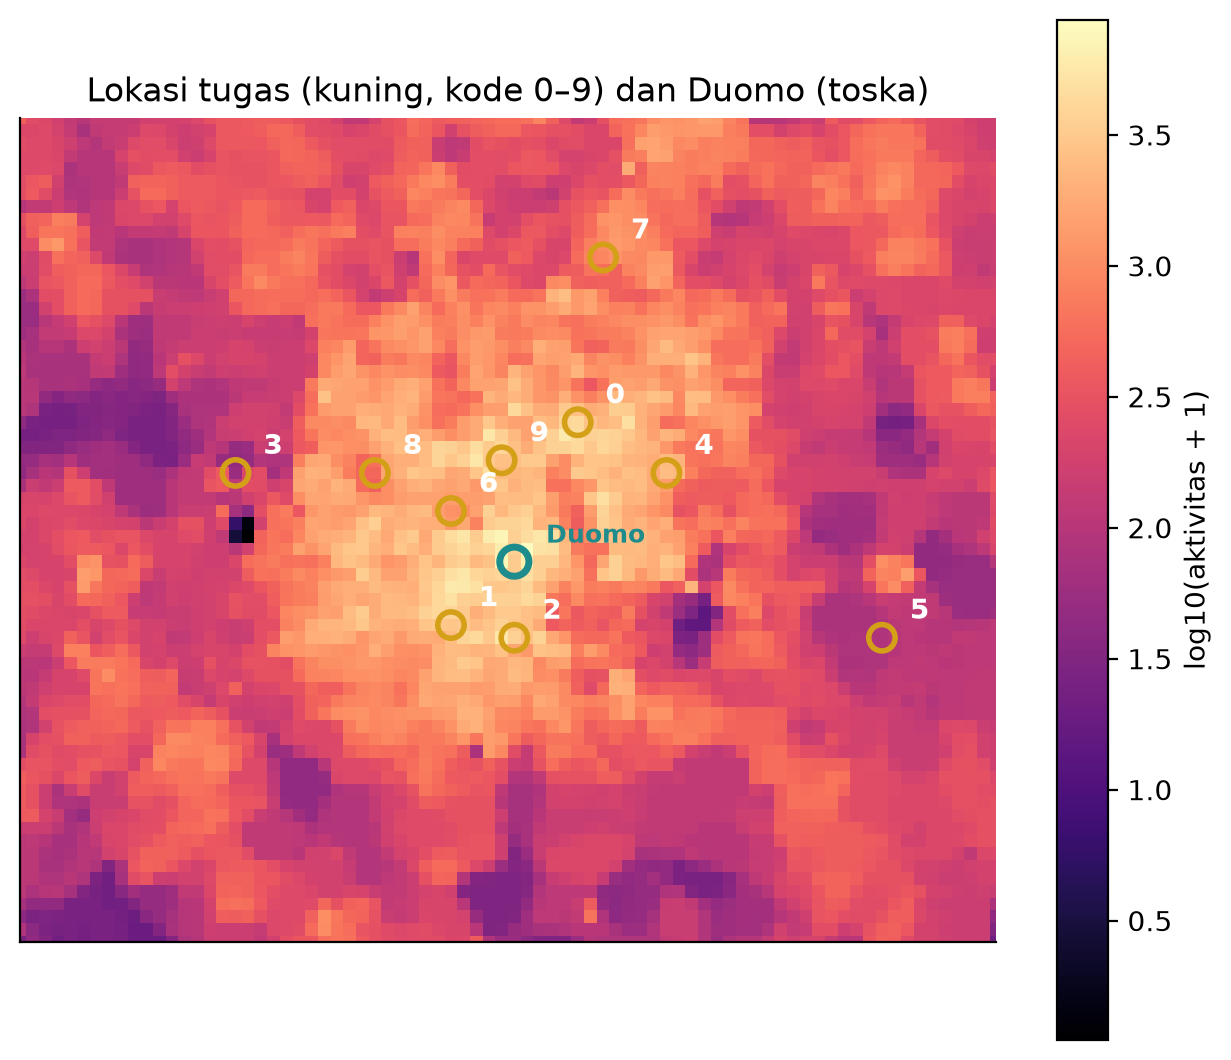
\includegraphics[width=\linewidth]{peta_lokasi_tugas.png}
  \caption{Peta skematis 10 lokasi tugas (kuning, kode 0--9) dan lokasi acuan Duomo (toska, D) pada grid Milan. Penanda kode 1 adalah Navigli (Darsena).}
  \label{fig:peta}
\end{figure}

\subsection{Pembagian Data dan Praproses}
Data dibagi menurut waktu: latih 11 Nov--8 Des (28 hari, 672 sampel), validasi 9--15 Des, uji 16--22 Des, dan Natal 23--29 Des; minggu 4--10 Nov hanya menjadi konteks jendela. Fitur distandarisasi dengan rata-rata dan simpangan baku dari data sebelum minggu validasi, sehingga tidak ada informasi masa depan yang bocor. Sampel dibentuk dengan \textit{windowing}: $W$ jam terakhir sebagai masukan dan jam berikutnya sebagai target, dan sebuah sampel masuk ke satu pembagian menurut jam targetnya. Data deret waktu tidak diacak karena pengacakan memasukkan data masa depan ke set latih dan mengabaikan urutan waktu, sehingga galat yang diukur terlalu optimistis dibanding penggunaan nyata.

\subsection{Model dan Konfigurasi Acuan}
ANN meratakan jendela $W \times$ fitur menjadi satu vektor lalu melewati lapisan tersembunyi ReLU, sehingga jumlah parameternya tumbuh linear terhadap $W$. RNN, LSTM, dan GRU memproses jendela jam demi jam dengan bobot yang sama pada setiap langkah, lalu \textit{hidden state} jam terakhir masuk ke lapisan keluaran; jumlah parameternya tidak bergantung pada $W$. LSTM dan GRU memakai gerbang untuk mengatur aliran informasi dan gradien. Konfigurasi acuan ada di Tabel~\ref{tab:acuan}; ukuran \textit{hidden} dipilih agar parameter model rekuren sekitar 5,5 ribu.

\begin{table}[t]
  \centering
  \caption{Konfigurasi acuan}
  \label{tab:acuan}
  \begin{tabular}{@{}ll@{}}
    \toprule
    Hyperparameter & Nilai acuan \\
    \midrule
    Panjang jendela $W$ & 24 jam \\
    Horizon & 1 jam \\
    Ukuran hidden & ANN 32, RNN 68, LSTM 33, GRU 38 \\
    Jumlah lapisan & ANN 2, rekuren 1 \\
    Fitur & net, call, sms, jam, hari (7) \\
    Optimizer, \textit{learning rate} & Adam, $10^{-3}$ \\
    \textit{Batch size} & 64 \\
    Loss, \textit{dropout}, \textit{clipping} & MSE, 0, tidak ada \\
    \textit{Early stopping} & \textit{patience} 30, maks.\ 300 epoch \\
    \bottomrule
  \end{tabular}
\end{table}

\subsection{Protokol Ablasi dan Evaluasi}
Satu faktor diubah setiap kali: panjang jendela $W \in \{6, 12, 24, 48, 168\}$ (A1), \textit{hidden} $\in \{16, 32, 64, 128\}$ (A2), jumlah lapisan $\in \{1, 2, 3\}$ (A3), \textit{learning rate} $\in \{10^{-4}, 10^{-3}, 10^{-2}\}$ (A4), dan kelompok fitur (net; net+call+sms; net+waktu; semua) (A5). Dua faktor pilihan dengan hipotesis tertulis sebelum dijalankan: dropout $\in \{0; 0{,}2; 0{,}5\}$ (B2) dan \textit{gradient clipping} $\in \{$tanpa; $0{,}5$; $1{,}0\}$ pada \textit{learning rate} $10^{-2}$ (B7). Hipotesisnya:

\emph{B2.} Dropout 0,2 menurunkan val MAE ANN lebih besar daripada model rekuren, karena ANN punya parameter paling banyak relatif terhadap 672 sampel latih dan selisih val ke test terbesar di Bagian A. Dropout 0,5 memperburuk model rekuren karena kapasitasnya kecil (sekitar 5 ribu parameter) sehingga \textit{underfit}.

\emph{B7.} \textit{Clipping} 0,5 dan 1,0 menurunkan val MAE dan simpangan baku RNN pada \textit{learning rate} 0,01 (acuan A4: val MAE 227,2 $\pm$ 6,4), karena RNN \textit{vanilla} rentan gradien meledak. Pengaruhnya pada LSTM dan GRU lebih kecil karena gerbangnya sudah menstabilkan gradien.

Dua faktor lain, ukuran \textit{batch} $\in \{16, 64, 256\}$ (B1) dan fungsi \textit{loss} $\in \{$MSE, MAE, Huber$\}$ (B4), dijalankan lebih dulu tanpa hipotesis tertulis, sehingga diperlakukan sebagai eksplorasi tambahan.

Setiap konfigurasi dilatih dengan seed 0, 1, 2 dan dilaporkan sebagai rata-rata $\pm$ simpangan baku. \textit{Early stopping} memakai val MSE untuk semua fungsi \textit{loss} agar adil. Metrik adalah MAE, RMSE, dan MAPE pada skala asli. Konfigurasi terbaik tiap model dipilih dengan val MAE; minggu uji dan Natal hanya untuk pelaporan. Pelatihan dilakukan di CPU \isi{spesifikasi laptop} dengan PyTorch 2.14.1, total waktu pelatihan 89,6 menit.

% ---------------------------------------------------------------------
\section{Hasil}

\subsection{Baseline Naif dan Acuan}
Tabel~\ref{tab:acuanhasil} memuat tiga baseline naif dan konfigurasi acuan di Duomo. Pada minggu uji, keempat model mengalahkan baseline naif terbaik (``minggu lalu'', 467,6) dengan selisih besar; RNN dan GRU terbaik, ANN terburuk. Di minggu Natal gambarnya berbeda: ANN (680,1), LSTM (586,0), dan GRU (468,2) lebih buruk daripada baseline ``nilai terakhir'' (431,2), dan hanya RNN (421,2) setara dengannya.

\begin{table}[t]
  \centering
  \caption{MAE baseline naif dan konfigurasi acuan di Duomo (rata-rata $\pm$ simpangan baku, 3 seed). Parameter: ANN 6.497, RNN 5.305, LSTM 5.578, GRU 5.397.}
  \label{tab:acuanhasil}
  \scriptsize
  \setlength{\tabcolsep}{3pt}
  \begin{tabular}{@{}lccc@{}}
    \toprule
    Metode & Val & Uji & Natal \\
    \midrule
    Naif: terakhir  & 662,6 & 600,9 & 431,2 \\
    Naif: kemarin   & 595,3 & 552,2 & 921,5 \\
    Naif: mgg lalu  & 492,8 & 467,6 & 1426,2 \\
    \midrule
    ANN  & $248{,}9 \pm 8{,}9$ & $309{,}9 \pm 5{,}9$ & $680{,}1 \pm 52{,}0$ \\
    RNN  & $206{,}1 \pm 7{,}4$ & $229{,}6 \pm 5{,}1$ & $421{,}2 \pm 2{,}4$ \\
    LSTM & $230{,}5 \pm 12{,}2$ & $273{,}6 \pm 25{,}4$ & $586{,}0 \pm 56{,}8$ \\
    GRU  & $207{,}5 \pm 3{,}8$ & $237{,}2 \pm 9{,}3$ & $468{,}2 \pm 21{,}8$ \\
    \bottomrule
  \end{tabular}
\end{table}

\subsection{Ablasi Wajib}
Tabel~\ref{tab:ablasi} merangkum val MAE seluruh ablasi (angka tebal: terendah dalam kelompok faktor untuk model itu).

\begin{table*}[t]
  \centering
  \caption{Val MAE (rata-rata $\pm$ simpangan baku, 3 seed) untuk setiap faktor ablasi di Duomo. Tebal = rata-rata terendah dalam kelompok faktor untuk model tersebut; selisih yang lebih kecil dari simpangan baku tidak dianggap nyata. Ukuran \textit{hidden} acuan adalah ANN 32, RNN 68, LSTM 33, GRU 38. Nilai acuan: $W=24$, lapisan ANN 2/rekuren 1, \textit{lr} $10^{-3}$, fitur ``semua'', \textit{batch} 64, loss MSE.}
  \label{tab:ablasi}
  \footnotesize
  \begin{tabular}{@{}llcccc@{}}
    \toprule
    Faktor & Nilai & ANN & RNN & LSTM & GRU \\
    \midrule
    A1: $W$ (jam) & 6   & $\mathbf{211{,}5 \pm 6{,}2}$ & $215{,}5 \pm 4{,}1$ & $\mathbf{227{,}1 \pm 4{,}3}$ & $212{,}6 \pm 11{,}5$ \\
                  & 12  & $238{,}5 \pm 4{,}5$ & $206{,}7 \pm 6{,}2$ & $235{,}6 \pm 2{,}0$ & $208{,}9 \pm 10{,}4$ \\
                  & 24  & $248{,}9 \pm 8{,}9$ & $206{,}1 \pm 7{,}4$ & $230{,}5 \pm 12{,}2$ & $207{,}5 \pm 3{,}8$ \\
                  & 48  & $262{,}6 \pm 3{,}8$ & $\mathbf{200{,}1 \pm 5{,}3}$ & $249{,}1 \pm 21{,}8$ & $\mathbf{206{,}7 \pm 5{,}0}$ \\
                  & 168 & $298{,}2 \pm 18{,}2$ & $204{,}8 \pm 10{,}2$ & $241{,}4 \pm 8{,}1$ & $\mathbf{206{,}7 \pm 5{,}1}$ \\
    \midrule
    A2: \textit{hidden} & 16  & $257{,}6 \pm 28{,}0$ & $247{,}0 \pm 5{,}8$ & $244{,}3 \pm 18{,}3$ & $216{,}8 \pm 21{,}2$ \\
                        & 32  & $248{,}9 \pm 8{,}9$ & $218{,}7 \pm 6{,}6$ & $241{,}5 \pm 20{,}5$ & $210{,}2 \pm 0{,}8$ \\
                        & 64  & $238{,}4 \pm 16{,}5$ & $\mathbf{207{,}2 \pm 12{,}8}$ & $218{,}1 \pm 1{,}9$ & $198{,}4 \pm 9{,}2$ \\
                        & 128 & $\mathbf{233{,}8 \pm 1{,}9}$ & $207{,}7 \pm 7{,}2$ & $\mathbf{207{,}1 \pm 8{,}4}$ & $\mathbf{188{,}7 \pm 4{,}2}$ \\
    \midrule
    A3: lapisan & 1 & $\mathbf{240{,}9 \pm 7{,}5}$ & $\mathbf{206{,}1 \pm 7{,}4}$ & $\mathbf{230{,}5 \pm 12{,}2}$ & $207{,}5 \pm 3{,}8$ \\
                & 2 & $248{,}9 \pm 8{,}9$ & $207{,}3 \pm 9{,}1$ & $254{,}8 \pm 14{,}5$ & $\mathbf{203{,}3 \pm 9{,}6}$ \\
                & 3 & $249{,}3 \pm 11{,}7$ & $225{,}1 \pm 12{,}7$ & $338{,}9 \pm 16{,}9$ & $212{,}2 \pm 15{,}9$ \\
    \midrule
    A4: \textit{lr} & $10^{-4}$ & $295{,}4 \pm 4{,}7$ & $285{,}0 \pm 13{,}7$ & $399{,}4 \pm 25{,}0$ & $398{,}4 \pm 8{,}6$ \\
                    & $10^{-3}$ & $\mathbf{248{,}9 \pm 8{,}9}$ & $\mathbf{206{,}1 \pm 7{,}4}$ & $230{,}5 \pm 12{,}2$ & $\mathbf{207{,}5 \pm 3{,}8}$ \\
                    & $10^{-2}$ & $261{,}8 \pm 16{,}6$ & $227{,}2 \pm 6{,}4$ & $\mathbf{215{,}9 \pm 14{,}2}$ & $208{,}2 \pm 5{,}6$ \\
    \midrule
    A5: fitur & net          & $260{,}5 \pm 7{,}0$ & $245{,}2 \pm 5{,}8$ & $266{,}2 \pm 5{,}7$ & $264{,}6 \pm 7{,}0$ \\
              & net+call+sms & $259{,}9 \pm 5{,}2$ & $224{,}1 \pm 2{,}3$ & $243{,}7 \pm 7{,}1$ & $231{,}8 \pm 12{,}6$ \\
              & net+waktu    & $\mathbf{246{,}0 \pm 9{,}8}$ & $223{,}0 \pm 9{,}5$ & $231{,}1 \pm 4{,}3$ & $213{,}2 \pm 18{,}2$ \\
              & semua        & $248{,}9 \pm 8{,}9$ & $\mathbf{206{,}1 \pm 7{,}4}$ & $\mathbf{230{,}5 \pm 12{,}2}$ & $\mathbf{207{,}5 \pm 3{,}8}$ \\
    \midrule
    B1: \textit{batch} & 16  & $\mathbf{244{,}4 \pm 17{,}4}$ & $\mathbf{202{,}4 \pm 8{,}8}$ & $\mathbf{209{,}2 \pm 18{,}7}$ & $\mathbf{202{,}3 \pm 4{,}3}$ \\
                       & 64  & $248{,}9 \pm 8{,}9$ & $206{,}1 \pm 7{,}4$ & $230{,}5 \pm 12{,}2$ & $207{,}5 \pm 3{,}8$ \\
                       & 256 & $254{,}5 \pm 13{,}2$ & $228{,}3 \pm 17{,}4$ & $269{,}6 \pm 10{,}8$ & $233{,}8 \pm 15{,}6$ \\
    \midrule
    B4: \textit{loss} & MSE   & $248{,}9 \pm 8{,}9$ & $\mathbf{206{,}1 \pm 7{,}4}$ & $\mathbf{230{,}5 \pm 12{,}2}$ & $\mathbf{207{,}5 \pm 3{,}8}$ \\
                      & MAE   & $\mathbf{238{,}4 \pm 5{,}3}$ & $217{,}9 \pm 9{,}3$ & $239{,}8 \pm 7{,}6$ & $213{,}5 \pm 14{,}7$ \\
                      & Huber & $241{,}9 \pm 3{,}7$ & $206{,}3 \pm 10{,}0$ & $233{,}6 \pm 13{,}6$ & $207{,}8 \pm 5{,}1$ \\
    \midrule
    B2: \textit{dropout} & 0   & $\mathbf{248{,}9 \pm 8{,}9}$ & $\mathbf{206{,}1 \pm 7{,}4}$ & $\mathbf{230{,}5 \pm 12{,}2}$ & $207{,}5 \pm 3{,}8$ \\
                         & 0,2 & $274{,}4 \pm 32{,}0$ & $239{,}5 \pm 10{,}7$ & $231{,}8 \pm 9{,}3$ & $\mathbf{203{,}9 \pm 5{,}1}$ \\
                         & 0,5 & $377{,}7 \pm 13{,}1$ & $254{,}8 \pm 11{,}1$ & $247{,}4 \pm 6{,}5$ & $259{,}5 \pm 29{,}0$ \\
    \midrule
    B7: \textit{clip} (\textit{lr} $10^{-2}$) & tanpa & $261{,}8 \pm 16{,}6$ & $\mathbf{227{,}2 \pm 6{,}4}$ & $215{,}9 \pm 14{,}2$ & $\mathbf{208{,}2 \pm 5{,}6}$ \\
                         & 0,5 & $250{,}6 \pm 15{,}9$ & $234{,}4 \pm 0{,}6$ & $\mathbf{213{,}3 \pm 4{,}0}$ & $217{,}5 \pm 17{,}0$ \\
                         & 1,0 & $\mathbf{248{,}7 \pm 7{,}0}$ & $231{,}7 \pm 2{,}6$ & $223{,}8 \pm 20{,}9$ & $210{,}6 \pm 9{,}5$ \\
    \bottomrule
  \end{tabular}
\end{table*}


\textbf{A1 (jendela).} ANN memburuk monoton terhadap $W$: val MAE $211{,}5$ ($W=6$) menjadi $298{,}2$ ($W=168$), sementara parameternya naik dari 2.465 ke 38.753 dan selisih uji--val naik dari 57,9 ke 103,8. RNN ($200{,}1$--$215{,}5$) dan GRU ($206{,}7$--$212{,}6$) hampir datar; hasil GRU untuk $W=48$ dan $W=168$ praktis identik pada setiap seed (selisih val MAE di bawah 0,05), sehingga informasi lebih dari 48 jam ke belakang hampir tidak memengaruhi keluarannya; LSTM ($227{,}1$--$249{,}1$) tanpa tren jelas. ANN dengan $W=6$ ($211{,}5$) setara RNN acuan ($206{,}1$). Gambar~\ref{fig:a1}.

\begin{figure}[t]
  \centering
  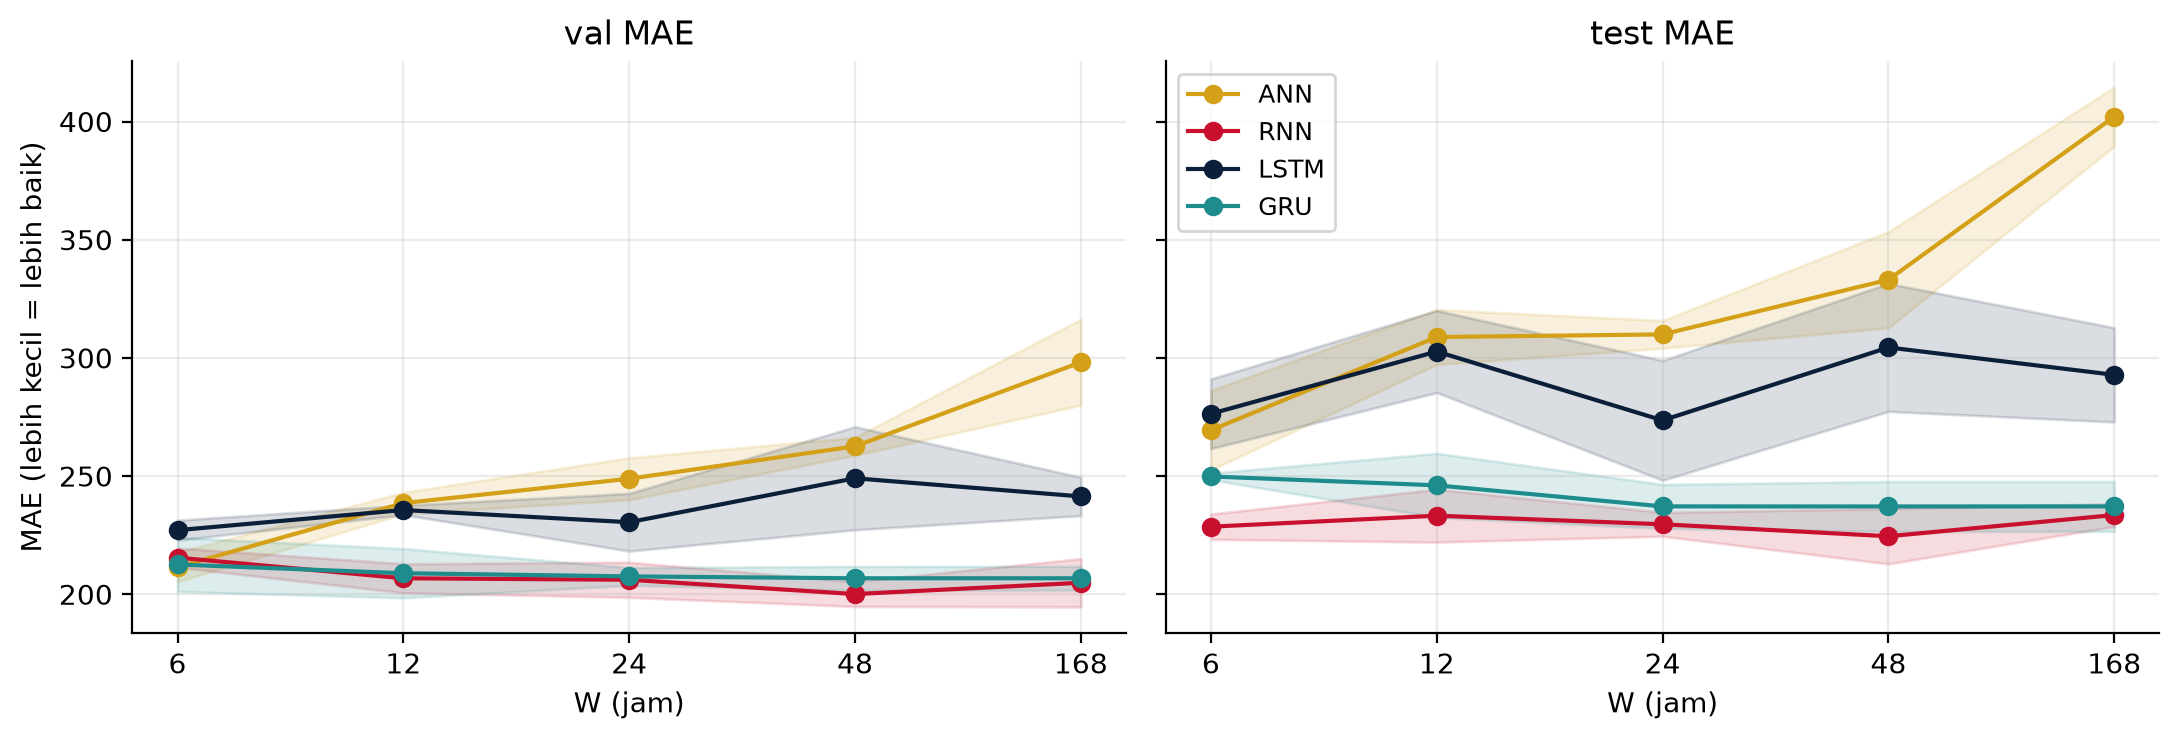
\includegraphics[width=\linewidth]{A1_W.png}
  \caption{Pengaruh panjang jendela $W$ terhadap val MAE (kiri) dan test MAE (kanan); area = $\pm 1$ simpangan baku.}
  \label{fig:a1}
\end{figure}

\textbf{A2 (\textit{hidden}).} Val MAE turun seiring \textit{hidden} untuk semua model, paling jelas pada GRU ($216{,}8 \to 188{,}7$). RNN mendatar sejak \textit{hidden} 64 ($207{,}2$ vs $207{,}7$ pada 128). GRU berukuran 32 (3.969 parameter, $210{,}2 \pm 0{,}8$) mengalahkan ANN berukuran 128 (38.273 parameter, $233{,}8 \pm 1{,}9$), dan RNN berukuran 64 (4.737) setara LSTM berukuran 128 (70.273): $207{,}2$ vs $207{,}1$ (Gambar~\ref{fig:a2}).

\begin{figure}[t]
  \centering
  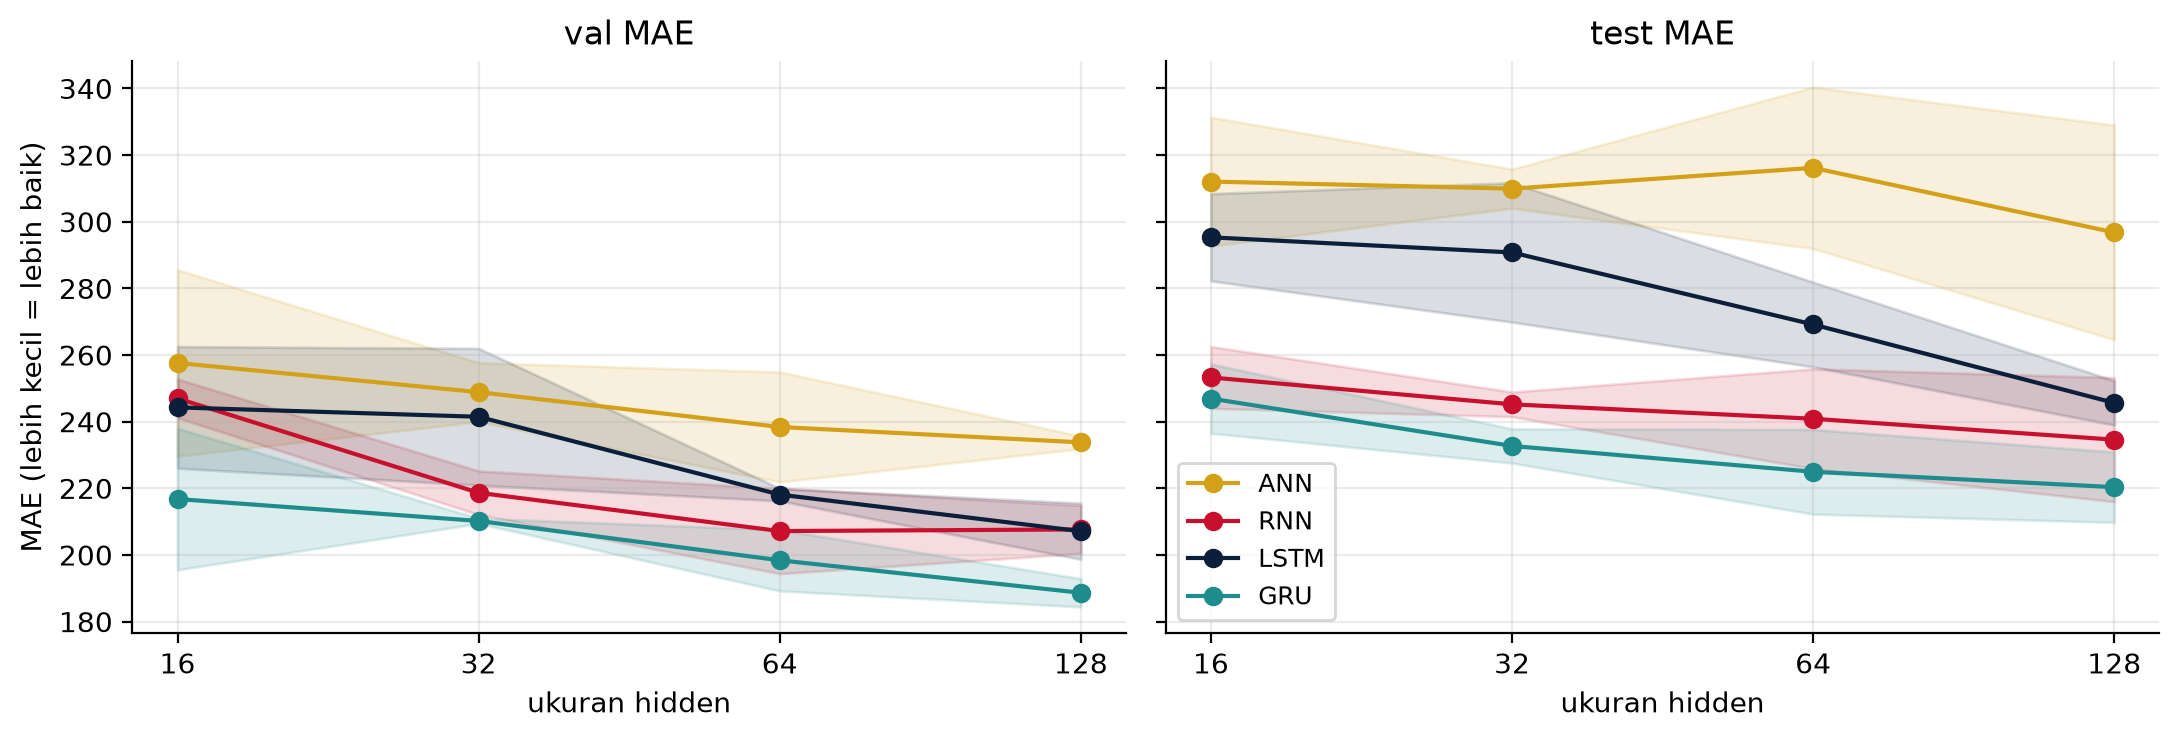
\includegraphics[width=\linewidth]{A2_hidden.png}
  \caption{Pengaruh ukuran \textit{hidden} terhadap val dan test MAE.}
  \label{fig:a2}
\end{figure}

\textbf{A3 (lapisan).} Lapisan tambahan tidak membantu. LSTM memburuk tegas ($230{,}5 \to 254{,}8 \to 338{,}9$; epoch rata-rata $168{,}7 \to 134{,}0$ dari satu ke tiga lapis), RNN tiga lapis memburuk ($225{,}1$), GRU dua lapis ($203{,}3 \pm 9{,}6$) tidak berbeda dari satu lapis ($207{,}5 \pm 3{,}8$), dan ANN datar.

\textbf{A4 (\textit{learning rate}).} Pada $10^{-4}$ semua model mencapai batas 300 epoch dan val MAE tinggi ($285{,}0$--$399{,}4$), jadi belum konvergen. Pada $10^{-2}$ epoch turun ke 62--68. LSTM membaik (val $215{,}9 \pm 14{,}2$; uji $225{,}8 \pm 4{,}2$ vs $273{,}6 \pm 25{,}4$), RNN dan ANN memburuk ($227{,}2$; $261{,}8$), GRU setara ($208{,}2$). Simpangan baku uji ANN naik dari 5,9 ke 53,2 dan RNN dari 5,1 ke 12,3, tetapi LSTM justru turun (25,4 ke 4,2) dan GRU hampir sama, jadi ketidakstabilan pada \textit{learning rate} besar tidak berlaku untuk semua model.

\textbf{A5 (fitur).} Hanya \textit{net} paling buruk untuk model rekuren (RNN $245{,}2$; GRU $264{,}6$; LSTM $266{,}2$). Menambah call+sms atau fitur waktu masing-masing membantu, dan gabungan (semua) terbaik untuk RNN, LSTM, dan GRU. Pada ANN hanya fitur waktu yang membantu ($246{,}0$); call+sms tidak ($259{,}9$ vs $260{,}5$).

\subsection{Ablasi Pilihan}
\textbf{B1 (\textit{batch}, eksploratif).} \textit{Batch} 16 memberi val MAE terendah pada keempat model; untuk ANN dan RNN selisihnya dari acuan (4,5 dan 3,7) kurang dari satu simpangan baku, GRU (5,2) sedikit di atasnya, dan hanya LSTM ($209{,}2$ vs $230{,}5$; selisih 21,3) jelas lebih besar. \textit{Batch} 256 terburuk (RNN $228{,}3$; LSTM $269{,}6$; GRU $233{,}8$) dan GRU mencapai batas 300 epoch pada ketiga seed. \textit{Batch} 16 juga lebih cepat daripada 64 karena membutuhkan lebih sedikit epoch (mis.\ GRU 41,1 s vs 59,5 s per run; epoch rata-rata 112 vs 194), sedangkan \textit{batch} 256 tercepat per run (GRU 19,3 s) tetapi tidak konvergen.

\textbf{B4 (\textit{loss}, eksploratif).} Menurut val MAE, \textit{loss} MAE hanya membantu ANN ($238{,}4$ vs $248{,}9$). RNN, LSTM, dan GRU terbaik dengan MSE, dengan Huber setara MSE dan MAE lebih buruk ($217{,}9$; $239{,}8$; $213{,}5$). Namun test MAE berlawanan untuk RNN ($207{,}1 \pm 6{,}5$ dengan MAE vs $229{,}6 \pm 5{,}1$ dengan MSE) dan GRU ($220{,}6 \pm 12{,}0$ vs $237{,}2 \pm 9{,}3$). Sesuai aturan, saya tidak memilih berdasarkan test. Untuk RMSE di validasi, MSE terbaik atau setara pada RNN ($309{,}3$), LSTM ($331{,}4$), dan GRU ($303{,}3$), sedangkan MAE terburuk ($339{,}6$; $350{,}5$; $331{,}0$), sesuai dugaan bahwa \textit{loss} MSE menyasar RMSE; hanya ANN yang lebih baik dengan MAE ($359{,}3$ vs $372{,}4$).

\textbf{B2 (\textit{dropout}).} Hipotesis pertama (dropout 0,2 membantu ANN lebih besar daripada model rekuren) \emph{tidak terbukti}: val MAE ANN justru naik dari $248{,}9$ ke $274{,}4$, RNN naik ke $239{,}5$, LSTM tidak berubah ($231{,}8$), dan hanya GRU yang sedikit membaik ($203{,}9 \pm 5{,}1$ vs $207{,}5 \pm 3{,}8$), selisih yang masih dalam simpangan baku. Hipotesis kedua (dropout 0,5 memperburuk model rekuren karena \textit{underfit}) \emph{terbukti}: RNN $254{,}8$, LSTM $247{,}4$, GRU $259{,}5$. Namun ANN yang paling terpukul ($377{,}7$), jadi pelemahan oleh dropout tinggi tidak khas untuk model rekuren.

\textbf{B7 (\textit{clipping}).} Hipotesis \emph{terbukti sebagian}. Simpangan baku val RNN turun dari 6,4 (tanpa \textit{clipping}) menjadi 0,6 (\textit{clip} 0,5) dan 2,6 (\textit{clip} 1,0), tetapi val MAE-nya tidak membaik ($227{,}2 \to 234{,}4$ dan $231{,}7$), meskipun test MAE membaik ($245{,}8 \to 229{,}8$ dan $231{,}4$; tidak dipakai untuk memilih). Pada LSTM dan GRU pengaruhnya kecil dan masih dalam simpangan baku (LSTM $215{,}9 \to 213{,}3$ dan $223{,}8$; GRU $208{,}2 \to 217{,}5$ dan $210{,}6$), sesuai dugaan bahwa gerbang sudah menstabilkan gradien. RNN dengan \textit{clipping} pada \textit{lr} $10^{-2}$ tetap lebih buruk daripada acuan \textit{lr} $10^{-3}$ ($206{,}1$).

\subsection{Konfigurasi Terbaik}
Langkah pertama mengikuti petunjuk: tiap model memakai gabungan nilai terbaik dari semua faktor (ANN: $W=6$, \textit{hidden} 128, 1 lapisan, fitur net+waktu, \textit{batch} 16, \textit{loss} MAE; RNN: $W=48$, \textit{batch} 16; LSTM: $W=6$, \textit{hidden} 128, \textit{lr} $10^{-2}$, \textit{batch} 16, \textit{clip} 0,5; GRU: $W=48$, \textit{hidden} 128, 2 lapisan, \textit{batch} 16, dropout 0,2). Hasilnya (baris ``gabungan'' di Tabel~\ref{tab:c}, percobaan C-coba1) lebih buruk daripada acuan pada val MAE untuk RNN, LSTM, dan GRU, dan lebih buruk daripada satu faktor tunggal terbaik pada keempat model. Sesuai petunjuk, konfigurasi akhir lalu dipilih dengan val MAE terendah di antara semua konfigurasi Duomo yang sudah dijalankan; hasilnya selalu satu faktor tunggal: $W=6$ untuk ANN, $W=48$ untuk RNN, \textit{hidden} 128 untuk LSTM dan GRU. Semua percobaan dilaporkan.

\begin{table}[t]
  \centering
  \caption{Acuan, gabungan semua nilai terbaik (C-coba1), dan konfigurasi terbaik terpilih (val MAE terendah) di Duomo. MAE, rata-rata $\pm$ simpangan baku, 3 seed.}
  \label{tab:c}
  \scriptsize
  \setlength{\tabcolsep}{2.5pt}
  \begin{tabular}{@{}llccc@{}}
    \toprule
    Model & Konfigurasi & Val & Uji & Natal \\
    \midrule
    ANN  & acuan & $248{,}9 \pm 8{,}9$ & $309{,}9 \pm 5{,}9$ & $680{,}1 \pm 52{,}0$ \\
         & gabungan & $219{,}2 \pm 3{,}0$ & $257{,}4 \pm 8{,}0$ & $601{,}5 \pm 73{,}6$ \\
         & terbaik: $W=6$ & $\mathbf{211{,}5 \pm 6{,}2}$ & $269{,}4 \pm 16{,}8$ & $532{,}5 \pm 78{,}1$ \\
    RNN  & acuan & $206{,}1 \pm 7{,}4$ & $229{,}6 \pm 5{,}1$ & $421{,}2 \pm 2{,}4$ \\
         & gabungan & $209{,}5 \pm 3{,}2$ & $226{,}3 \pm 4{,}9$ & $385{,}4 \pm 13{,}8$ \\
         & terbaik: $W=48$ & $\mathbf{200{,}1 \pm 5{,}3}$ & $224{,}5 \pm 11{,}7$ & $404{,}5 \pm 9{,}9$ \\
    LSTM & acuan & $230{,}5 \pm 12{,}2$ & $273{,}6 \pm 25{,}4$ & $586{,}0 \pm 56{,}8$ \\
         & gabungan & $246{,}2 \pm 12{,}9$ & $247{,}3 \pm 12{,}1$ & $450{,}9 \pm 31{,}4$ \\
         & terbaik: \textit{hidden} 128 & $\mathbf{207{,}1 \pm 8{,}4}$ & $245{,}6 \pm 6{,}7$ & $491{,}1 \pm 7{,}6$ \\
    GRU  & acuan & $207{,}5 \pm 3{,}8$ & $237{,}2 \pm 9{,}3$ & $468{,}2 \pm 21{,}8$ \\
         & gabungan & $219{,}1 \pm 2{,}9$ & $240{,}7 \pm 15{,}4$ & $475{,}4 \pm 29{,}1$ \\
         & terbaik: \textit{hidden} 128 & $\mathbf{188{,}7 \pm 4{,}2}$ & $220{,}3 \pm 10{,}6$ & $435{,}2 \pm 7{,}5$ \\
    \bottomrule
  \end{tabular}
\end{table}

Pada minggu uji, konfigurasi terbaik menurunkan test MAE dari acuan sebesar 13,1\,\% (ANN), 2,2\,\% (RNN), 10,2\,\% (LSTM), dan 7,1\,\% (GRU); untuk RNN selisih itu lebih kecil daripada simpangan baku, jadi tidak dianggap nyata. GRU \textit{hidden} 128 memiliki val MAE terendah ($188{,}7$) dan test MAE terendah ($220{,}3$), tetapi selisihnya dari RNN $W=48$ ($224{,}5$) berada dalam simpangan baku. Pada minggu Natal, hanya RNN ($404{,}5$) yang di bawah baseline ``nilai terakhir'' ($431{,}2$); GRU ($435{,}2$) setara, LSTM ($491{,}1$) dan ANN ($532{,}5$) di atasnya (Gambar~\ref{fig:c}).

\begin{figure}[t]
  \centering
  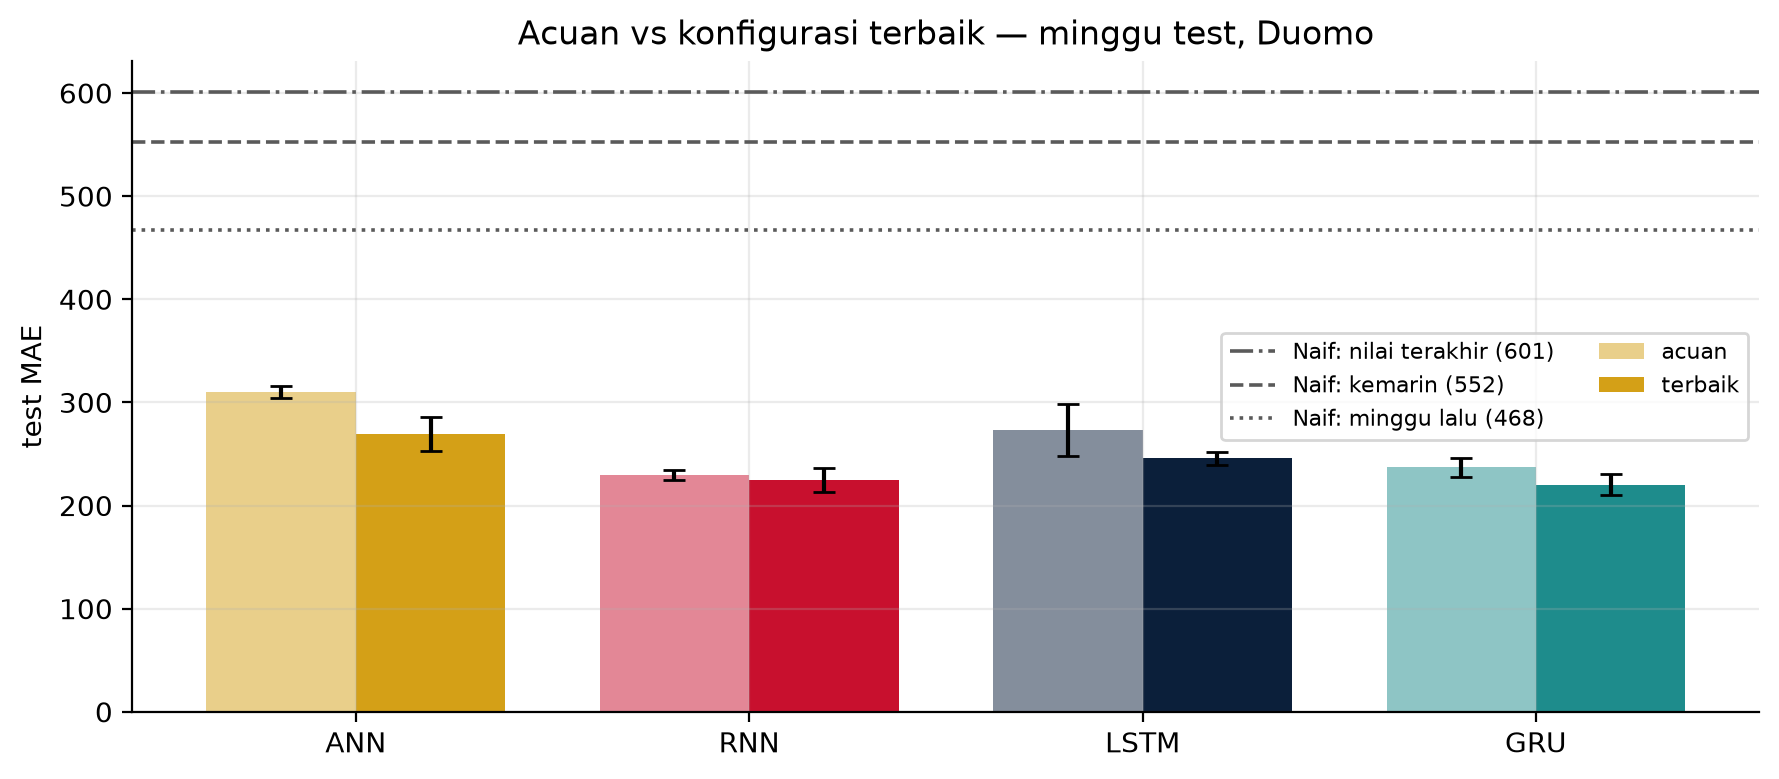
\includegraphics[width=\linewidth]{C_terbaik_vs_acuan.png}
  \caption{Test MAE acuan dan konfigurasi terbaik terhadap baseline naif, Duomo.}
  \label{fig:c}
\end{figure}

\subsection{Uji Generalisasi}
Tabel~\ref{tab:d} membandingkan konfigurasi acuan dan konfigurasi terbaik Duomo (dipakai tanpa diubah) di Navigli (Darsena). Pada minggu uji, keempat model mengalahkan baseline naif terbaik (``nilai terakhir'', 272,0). GRU ($190{,}8$) dan RNN ($193{,}0$) terbaik, disusul ANN ($222{,}3$) dan LSTM ($247{,}3$). Urutan ini berbeda dari Duomo: ANN tidak lagi terburuk, dan selisih ANN dengan LSTM masih dalam simpangan baku LSTM (54,3).

\begin{table}[t]
  \centering
  \caption{MAE di Navigli (Darsena), rata-rata $\pm$ simpangan baku, 3 seed. Baseline naif terbaik (val/uji/Natal): 225,7 / 272,0 / 177,7.}
  \label{tab:d}
  \scriptsize
  \setlength{\tabcolsep}{2.5pt}
  \begin{tabular}{@{}llccc@{}}
    \toprule
    Model & Konfigurasi & Val & Uji & Natal \\
    \midrule
    ANN  & acuan   & $166{,}6 \pm 5{,}3$ & $222{,}3 \pm 27{,}4$ & $664{,}5 \pm 190{,}8$ \\
         & terbaik & $148{,}5 \pm 5{,}3$ & $213{,}9 \pm 14{,}4$ & $688{,}7 \pm 151{,}3$ \\
    RNN  & acuan   & $147{,}3 \pm 4{,}9$ & $193{,}0 \pm 9{,}7$  & $534{,}7 \pm 148{,}9$ \\
         & terbaik & $144{,}8 \pm 3{,}1$ & $204{,}2 \pm 21{,}7$ & $548{,}8 \pm 100{,}9$ \\
    LSTM & acuan   & $164{,}3 \pm 9{,}3$ & $247{,}3 \pm 54{,}3$ & $950{,}8 \pm 110{,}9$ \\
         & terbaik & $153{,}8 \pm 0{,}9$ & $243{,}8 \pm 20{,}4$ & $839{,}5 \pm 35{,}7$ \\
    GRU  & acuan   & $149{,}0 \pm 6{,}0$ & $190{,}8 \pm 6{,}8$  & $496{,}4 \pm 50{,}9$ \\
         & terbaik & $139{,}0 \pm 3{,}9$ & $188{,}4 \pm 24{,}3$ & $620{,}8 \pm 81{,}7$ \\
    \bottomrule
  \end{tabular}
\end{table}

Konfigurasi terbaik Duomo menurunkan val MAE di Navigli pada ANN ($166{,}6 \to 148{,}5$), GRU ($149{,}0 \to 139{,}0$), dan sedikit pada LSTM ($164{,}3 \to 153{,}8$, hanya di atas simpangan baku), tetapi tidak pada RNN ($147{,}3 \to 144{,}8$). Manfaat itu tidak bertahan pada minggu uji: ANN ($222{,}3 \to 213{,}9$), LSTM ($247{,}3 \to 243{,}8$), dan GRU ($190{,}8 \to 188{,}4$) berubah dalam simpangan baku, sedangkan RNN justru naik ($193{,}0 \to 204{,}2$). Jadi kesimpulan dari Duomo bahwa konfigurasi terbaik lebih baik daripada acuan hanya berlaku sebagian di Navigli. Dugaan saya: konfigurasi dipilih pada satu lokasi dan satu minggu validasi sehingga tidak otomatis berpindah ke lokasi lain; hal ini tidak diuji lebih lanjut.

Pada minggu Natal, baseline ``nilai terakhir'' (177,7) mengalahkan semua model, yang galatnya sekitar tiga hingga lima kali lebih besar ($496{,}4$--$950{,}8$). Konfigurasi terbaik memperburuk GRU ($496{,}4 \to 620{,}8$) dan hanya LSTM yang membaik ($950{,}8 \to 839{,}5$). Gambar~\ref{fig:pola} menunjukkan pola yang berbeda: di Duomo puncak harian stabil di sekitar 6.000--9.000 dan hanya turun sekitar 24--26 Desember, sedangkan di Navigli puncak harian lebih rendah dan lebih tidak teratur (sekitar 3.500--6.000 dengan lonjakan sesekali), lalu turun ke sekitar 2.000--2.700 sepanjang minggu Natal tanpa pulih. Pola Navigli yang rendah dan datar itu sejalan dengan keunggulan baseline ``nilai terakhir'' pada Natal, tetapi hubungan sebabnya tidak saya uji.

\begin{figure}[t]
  \centering
  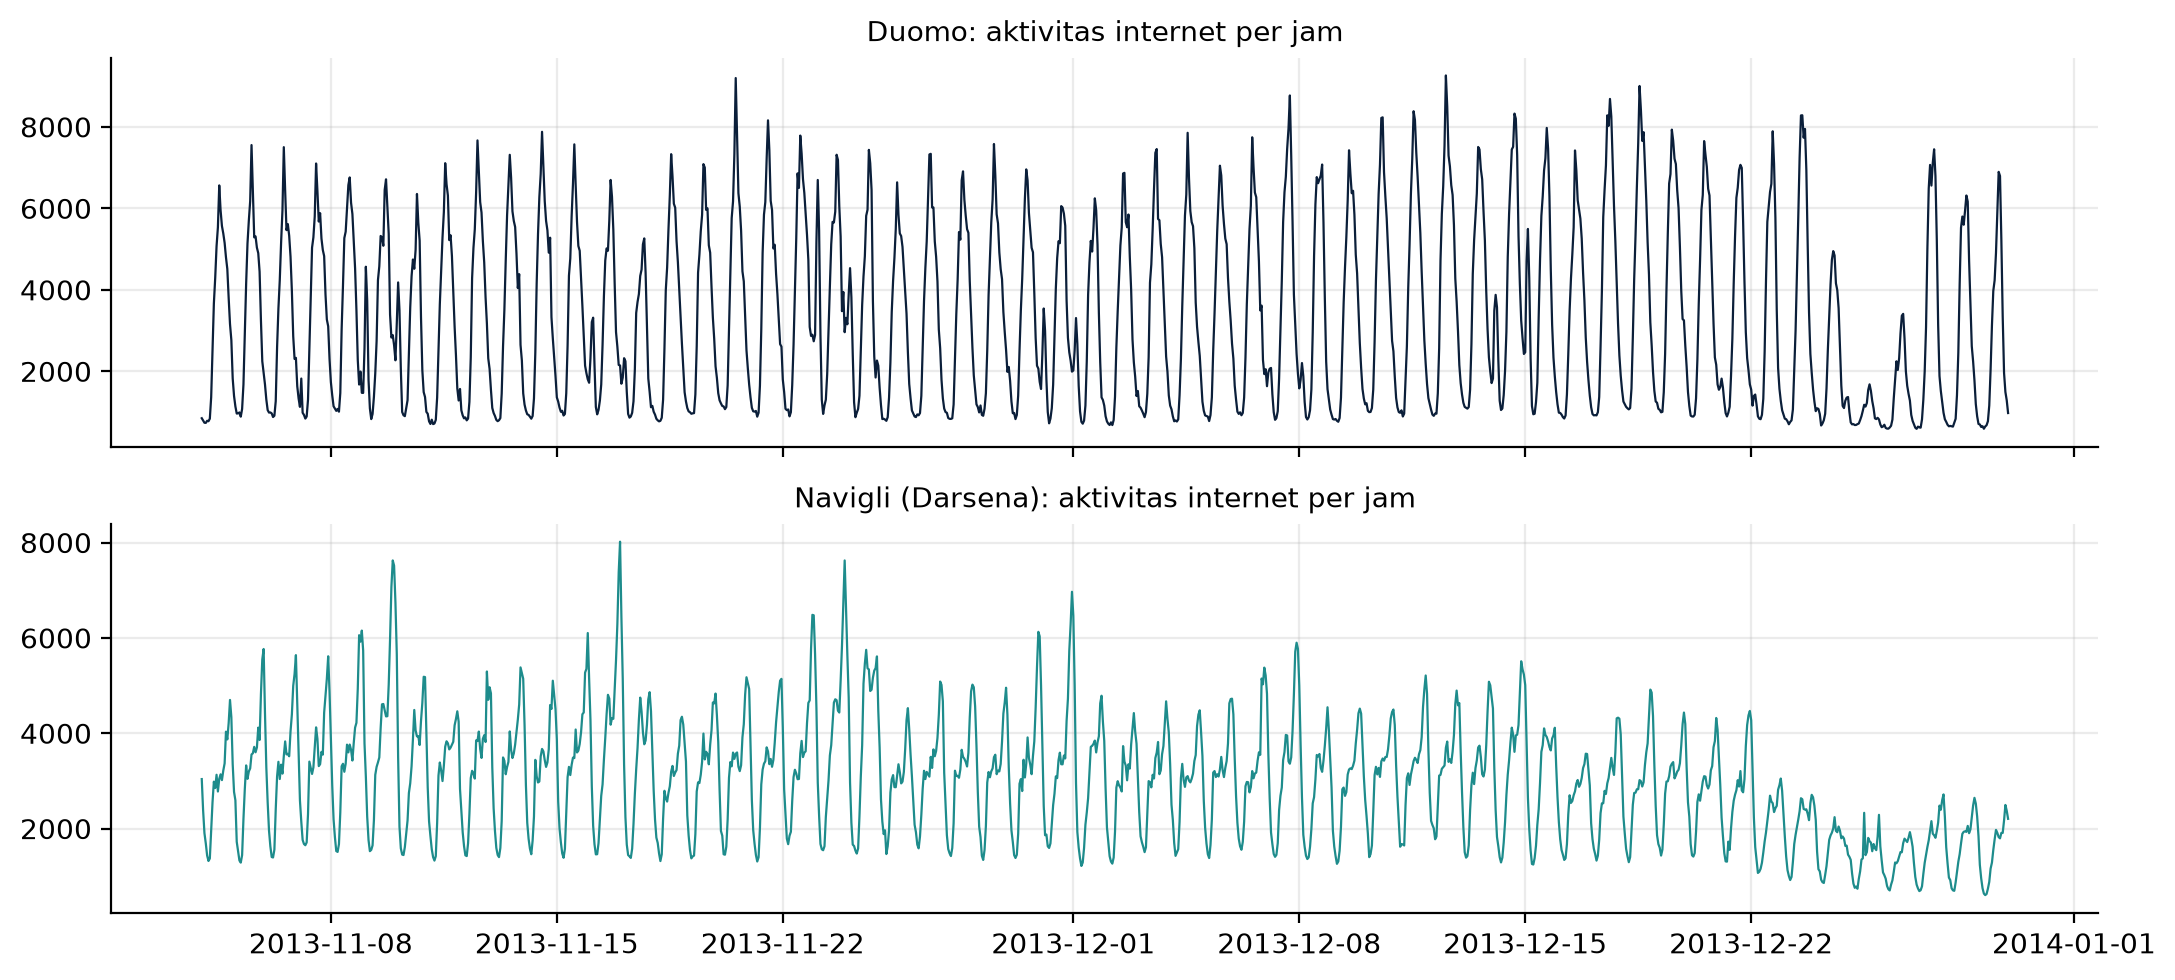
\includegraphics[width=\linewidth]{D_pola_lokasi.png}
  \caption{Aktivitas internet per jam di Duomo (atas) dan Navigli (bawah), 4 November--29 Desember 2013.}
  \label{fig:pola}
\end{figure}

% ---------------------------------------------------------------------
\section{Pembahasan}
\textbf{Struktur model lebih penting daripada jumlah parameter.} ANN meratakan jendela sehingga parameternya tumbuh linear terhadap $W$, sementara data latih hanya 672 sampel. Pola yang saya lihat konsisten dengan \textit{overfitting} (val MAE naik, epoch hingga \textit{early stopping} turun dari 166,7 ke 76,3, selisih uji--val membesar), meskipun saya tidak menguji penyebab itu secara langsung. Model rekuren memakai bobot yang sama di setiap langkah waktu, sehingga tidak terpengaruh $W$ dan GRU berukuran 32 sudah mengalahkan ANN yang hampir sepuluh kali lebih besar. Dugaan saya: kemiripan pola jam ke jam membuat struktur sekuensial menjadi prior yang menguntungkan pada data kecil.

\textbf{Faktor yang berpengaruh dan yang tidak.} Faktor yang menggerakkan hasil di luar noise: \textit{learning rate} terlalu kecil (tidak konvergen dalam 300 epoch), \textit{batch} besar (hanya sekitar tiga pembaruan per epoch sehingga GRU habis epoch), dan jumlah lapisan untuk LSTM. Dropout tidak membantu pada data sekecil ini (kecuali sedikit pada GRU), dan \textit{clipping} menstabilkan RNN pada \textit{learning rate} besar tanpa memperbaiki val MAE. Pengaruh fitur jelas, dan fitur waktu murah serta efektif karena $W=24$ tidak memuat pola mingguan. Perbedaan antar model rekuren (RNN, GRU) tidak lebih besar daripada simpangan baku antar seed (mis.\ uji $229{,}6 \pm 5{,}1$ vs $237{,}2 \pm 9{,}3$), jadi saya tidak mengklaim satu lebih baik; hanya ANN, dan umumnya LSTM, berbeda jelas. Mengapa LSTM memburuk dengan lapisan lebih banyak dan membaik pada \textit{learning rate} besar belum saya uji; kurva \textit{loss} diperlukan sebelum menyimpulkan.

\textbf{Nilai terbaik per faktor tidak dapat digabung begitu saja.} Gabungan nilai terbaik justru lebih buruk daripada satu faktor tunggal pada keempat model (mis.\ GRU $219{,}1$ vs $188{,}7$ dengan \textit{hidden} 128 saja; LSTM $246{,}2$ vs $207{,}1$). Dugaan saya: GRU gabungan memiliki 151.809 parameter (sekitar 28 kali acuan) dan LSTM gabungan memadukan \textit{lr} $10^{-2}$, \textit{batch} 16, dan \textit{clipping}, yang membuat pelatihan berhenti sangat dini (rata-rata 45 epoch), sehingga nilai yang baik satu per satu bersaing satu sama lain. Hal ini tidak diuji secara terpisah.

\textbf{Pemilihan dengan satu minggu validasi tidak stabil.} Pada B4, val menilai MAE lebih buruk untuk RNN sementara uji menilai jauh lebih baik. Perbedaan antar-minggu (val 9--15 Des vs uji 16--22 Des) membuat pemilihan memakai satu minggu bisa keliru; ini diperparah oleh \textit{early stopping} yang memakai val MSE, sehingga perbandingan \textit{loss} berdasarkan val MAE tidak sepenuhnya adil.

\textbf{Minggu Natal.} Galat Natal sekitar dua hingga tiga kali val (RNN $421{,}2$ vs $206{,}1$; ANN $680{,}1$ vs $248{,}9$). Data latih empat minggu tidak memuat pola libur sehingga model hanya bisa mengekstrapolasi. Baseline ``nilai terakhir'' ($431{,}2$) setara RNN dan mengalahkan model lain, jadi belajar dari data tanpa libur tidak otomatis lebih baik daripada tebakan sederhana pada kondisi di luar distribusi latih.

\textbf{Keterbatasan.} Satu kota dan satu lokasi utama; empat minggu latih; satu kali pembagian waktu; tiga seed (simpangan baku dari tiga titik sendiri tidak stabil); faktor diubah satu per satu sehingga interaksi tidak terukur; dan konfigurasi gabungan terbaik tidak dijamin terbaik bersama-sama.

% ---------------------------------------------------------------------
\section{Kesimpulan}
Pada konfigurasi acuan di Duomo, RNN dan GRU (test MAE $229{,}6$ dan $237{,}2$) lebih baik daripada ANN ($309{,}9$) dan baseline naif terbaik ($467{,}6$), dan GRU kecil mengalahkan ANN yang hampir sepuluh kali lebih besar. Faktor yang paling menggerakkan hasil adalah \textit{learning rate} yang terlalu kecil, \textit{batch} besar, kelompok fitur, dan panjang jendela pada ANN; dropout tidak membantu dan \textit{clipping} hanya menstabilkan RNN. Konfigurasi terbaik (GRU \textit{hidden} 128, test MAE $220{,}3 \pm 10{,}6$, turun $7{,}1$\,\% dari acuan GRU) tidak berbeda nyata dari RNN $W=48$, dan menggabungkan semua nilai terbaik justru lebih buruk daripada satu faktor terbaik. Di Navigli urutan model berubah dan konfigurasi terbaik Duomo tidak konsisten lebih baik pada minggu uji, sedangkan pada minggu Natal semua model kalah dari baseline ``nilai terakhir'' di Navigli dan hanya RNN yang setara dengannya di Duomo.

% ---------------------------------------------------------------------
\section*{Kontribusi}
Laporan dan seluruh eksperimen dikerjakan secara individu oleh Zahra Shakilla: menjalankan eksperimen, menganalisis hasil, dan menulis laporan.

\section*{Pernyataan Penggunaan AI}
Saya memakai Claude (Anthropic) untuk membantu pengaturan Git dan Jupyter, membaca dan memeriksa tabel hasil, Mengecek dan meminta bantuan untuk menelaah bagian bagian errornya. Seluruh angka berasal dari run saya sendiri di notebook, dan isi laporan telah saya periksa. 
\section*{Kode dan Data}
Kode, notebook beserta output, dan seluruh hasil run tersedia di \url{https://github.com/zahra124400021-glitch/dlw-tugas-ra-124400021}.

\begin{thebibliography}{4}
\bibitem{hochreiter1997lstm} S. Hochreiter dan J. Schmidhuber, "Long short-term memory," \textit{Neural Computation}, vol. 9, no. 8, pp. 1735--1780, 1997.
\bibitem{cho2014gru} K. Cho \textit{et al.}, "Learning phrase representations using RNN encoder--decoder for statistical machine translation," dalam \textit{Proc. EMNLP}, 2014, pp. 1724--1734.
\bibitem{barlacchi2015milan} G. Barlacchi \textit{et al.}, "A multi-source dataset of urban life in the city of Milan and the province of Trentino," \textit{Scientific Data}, vol. 2, art. 150055, 2015.
\bibitem{zhang2021fedda} C. Zhang, S. Dang, B. Shihada, dan M.-S. Alouini, "Dual attention-based federated learning for wireless traffic prediction," dalam \textit{IEEE INFOCOM}, 2021, pp. 1--10.
\end{thebibliography}

\end{document}
